%%
%% This is file `sample-sigconf.tex',
%% generated with the docstrip utility.
%%
%% The original source files were:
%%
%% samples.dtx  (with options: `all,proceedings,bibtex,sigconf')
%% 
%% IMPORTANT NOTICE:
%% 
%% For the copyright see the source file.
%% 
%% Any modified versions of this file must be renamed
%% with new filenames distinct from sample-sigconf.tex.
%% 
%% For distribution of the original source see the terms
%% for copying and modification in the file samples.dtx.
%% 
%% This generated file may be distributed as long as the
%% original source files, as listed above, are part of the
%% same distribution. (The sources need not necessarily be
%% in the same archive or directory.)
%%
%%
%% Commands for TeXCount
%TC:macro \cite [option:text,text]
%TC:macro \citep [option:text,text]
%TC:macro \citet [option:text,text]
%TC:envir table 0 1
%TC:envir table* 0 1
%TC:envir tabular [ignore] word
%TC:envir displaymath 0 word
%TC:envir math 0 word
%TC:envir comment 0 0
%%
%% The first command in your LaTeX source must be the \documentclass
%% command.
%%
%% For submission and review of your manuscript please change the
%% command to \documentclass[manuscript, screen, review]{acmart}.
%%
%% When submitting camera ready or to TAPS, please change the command
%% to \documentclass[sigconf]{acmart} or whichever template is required
%% for your publication.
%%
%%
\documentclass[sigconf, authorversion=true, nonacm=true]{acmart}%%
%% \BibTeX command to typeset BibTeX logo in the docs
\AtBeginDocument{%
  \providecommand\BibTeX{{%
    Bib\TeX}}}

%% Rights management information.  This information is sent to you
%% when you complete the rights form.  These commands have SAMPLE
%% values in them; it is your responsibility as an author to replace
%% the commands and values with those provided to you when you
%% complete the rights form.
\setcopyright{acmlicensed}
\copyrightyear{2018}
\acmYear{2018}
\acmDOI{XXXXXXX.XXXXXXX}
%% These commands are for a PROCEEDINGS abstract or paper.
\acmConference[Conference acronym 'XX]{Make sure to enter the correct
  conference title from your rights confirmation email}{June 03--05,
  2018}{Woodstock, NY}
%%
%%  Uncomment \acmBooktitle if the title of the proceedings is different
%%  from ``Proceedings of ...''!
%%
%%\acmBooktitle{Woodstock '18: ACM Symposium on Neural Gaze Detection,
%%  June 03--05, 2018, Woodstock, NY}
\acmISBN{978-1-4503-XXXX-X/2018/06}


%%
%% Submission ID.
%% Use this when submitting an article to a sponsored event. You'll
%% receive a unique submission ID from the organizers
%% of the event, and this ID should be used as the parameter to this command.
%%\acmSubmissionID{123-A56-BU3}

%%
%% For managing citations, it is recommended to use bibliography
%% files in BibTeX format.
%%
%% You can then either use BibTeX with the ACM-Reference-Format style,
%% or BibLaTeX with the acmnumeric or acmauthoryear sytles, that include
%% support for advanced citation of software artefact from the
%% biblatex-software package, also separately available on CTAN.
%%
%% Look at the sample-*-biblatex.tex files for templates showcasing
%% the biblatex styles.
%%

%%
%% The majority of ACM publications use numbered citations and
%% references.  The command \citestyle{authoryear} switches to the
%% "author year" style.
%%
%% If you are preparing content for an event
%% sponsored by ACM SIGGRAPH, you must use the "author year" style of
%% citations and references.
%% Uncommenting
%% the next command will enable that style.
%%\citestyle{acmauthoryear}


%%
%% end of the preamble, start of the body of the document source.
\begin{document}

%%
%% The "title" command has an optional parameter,
%% allowing the author to define a "short title" to be used in page headers.
\title{CyberEscape: Designing an Educational Escape Room for Cybersecurity Awareness}

%%
%% The "author" command and its associated commands are used to define
%% the authors and their affiliations.
%% Of note is the shared affiliation of the first two authors, and the
%% "authornote" and "authornotemark" commands
%% used to denote shared contribution to the research.
\author{Guilherme Mendes da Silva}
\affiliation{%
  \institution{University of Luxembourg}
  \city{Belval}
  \country{Luxembourg}
}


%%
%% By default, the full list of authors will be used in the page
%% headers. Often, this list is too long, and will overlap
%% other information printed in the page headers. This command allows
%% the author to define a more concise list
%% of authors' names for this purpose.
\renewcommand{\shortauthors}{Mendes}

%%
%% The abstract is a short summary of the work to be presented in the
%% article.
\begin{abstract}
Traditional cybersecurity awareness training programmes suffer from rapid knowledge decay and low engagement, leaving non-expert users vulnerable to attacks that exploit the human factor. This paper presents CyberEscape, a digital educational escape room (DEER) prototype designed to build cybersecurity awareness through active, scenario-based learning. Grounded in constructivist and situated learning principles, the prototype places players in three realistic threat scenarios: identifying phishing emails in a simulated inbox, evaluating password strength based on publicly visible personal information, and navigating safely on a public Wi-Fi network. The prototype was implemented in Python using the Pygame library, following a sequential checkpoint structure with immediate contextual feedback after each decision. This work demonstrates the feasibility of applying DEER mechanics to cybersecurity education and provides a documented design and working proof-of-concept prototype for further development and evaluation.
\end{abstract}

%%
%% The code below is generated by the tool at http://dl.acm.org/ccs.cfm.
%% Please copy and paste the code instead of the example below.
%%
\begin{CCSXML}
<ccs2012>
   <concept>
       <concept_id>10010405.10010489.10010495</concept_id>
       <concept_desc>Applied computing~E-learning</concept_desc>
       <concept_significance>500</concept_significance>
       </concept>
 </ccs2012>
\end{CCSXML}

\ccsdesc[500]{Applied computing~E-learning}
%%
%% Keywords. The author(s) should pick words that accurately describe
%% the work being presented. Separate the keywords with commas.
\keywords{Cybersecurity, Digital Educational Escape Rooms, Game-based learning}
%% A "teaser" image appears between the author and affiliation
%% information and the body of the document, and typically spans the
%% page.


% \received{20 February 2007}
% \received[revised]{12 March 2009}
% \received[accepted]{5 June 2009}

%%
%% This command processes the author and affiliation and title
%% information and builds the first part of the formatted document.
\maketitle

\section{Introduction}
The scale of the cybersecurity threat to everyday users and organisations has reached a critical threshold, with threat actors exploiting vulnerabilities at an increasingly rapid pace. According to the ENISA Threat Landscape 2025, phishing remains the dominant intrusion vector, accounting for approximately 60\% of observed cases and serving as a frequent precursor to the deployment of malicious code \cite{noauthor_threat_2025}. This landscape is further complicated by a 27\% year-on-year increase in newly disclosed vulnerabilities, totalling over 42,000 in the most recent reporting period \cite{noauthor_threat_2025}.


While technical security infrastructures continue to advance, cybercriminals have shifted their focus toward exploiting the "human factor," making non-expert users the primary target for attacks like phishing and social engineering \cite{keller_digital_2025}. Despite the necessity of effective Security Education, Training, and Awareness (SETA) programmes, traditional approaches remain largely passive, relying on online lectures, videos, and static tutorials that require participants to observe rather than actively learn \cite{keller_digital_2025, makri_digital_2021}. These methods can be perceived as uninspiring and tedious by learners, leading to low motivational potential and poor long-term retention of critical security competencies \cite{keller_digital_2025}. These methods are frequently perceived as uninspiring and tedious, leading to low motivational potential and rapid knowledge decay, where training increments often evaporate within 15 to 30 days How effective are SETA programmes.


Although game-based learning has emerged as a promising strategy to improve engagement, digital educational escape rooms (DEERs) specifically remain a relatively under-explored area for cybersecurity education \cite{keller_digital_2025}. Most existing research has focused on the pedagogical aspects of physical escape rooms, leaving a notable gap in understanding how fully digital, immersive escape environments can be used to foster specific cybersecurity skills \cite{makri_digital_2021}.


This paper proposes and documents CyberEscape, a digital educational escape room that immerses users in realistic cybersecurity scenarios to build awareness through active decision-making and immediate feedback. By placing learners in a "safe" virtual environment where they can experience the immediate consequences of their choices.


The remainder of this paper is structured as follows. Section 2 reviews related work on game-based learning and cybersecurity education. Section 3 analyses the cyberattack landscape and justifies the selected threat scenarios. Section 4 presents the design of the escape room. Section 5 describes the prototype implementation. Section 6 concludes the paper.

\section{Related work}

\subsection{Game-based learning}

Game-based learning (GBL) refers to the use of games as instructional tools where learning objectives are inherently integrated into the game structure \cite{keller_digital_2025, plass_handbook_2020, plass_foundations_2015}. Research has consistently shown that GBL produces superior learning outcomes compared to conventional teaching methods; for example, students in a GBL group achieved significantly higher learning gains than a control group, with a statistical significance of p<0.05 \cite{wardoyo_effectiveness_2020}. A core advantage of this approach is the concept of "graceful failure," where the game acts as a "safe space" that treats mistakes as necessary, low-consequence steps in the learning process rather than final negative outcomes \cite{keller_digital_2025, plass_handbook_2020, plass_foundations_2015}. This environment fosters the inner drive of a player, or intrinsic motivation \cite{plass_handbook_2020, plass_foundations_2015}. When applied as educational escape rooms, GBL leverages high situational interest to engage participants in active problem-solving and decision-making under time pressure \cite{makri_digital_2021}. These characteristics transform learners from passive receivers of information into active participants, making the format especially relevant for cybersecurity, where users must practice recognising and responding to realistic threats in a risk-free environment \cite{makri_digital_2021},for example, emotions like urgency or fear might be replicated by the time constraints of an escape room.

\subsection{Escape Rooms in Education}


An Educational Escape Room (EER) is a game, generally team-based, filled with puzzles to be solved in a determinate amount of time \cite{wiemker_elumir_clare_escape_room_2015} with the goal of gaining knowledge in a subject or even developing domain specific skills \cite{veldkamp_escape_2020} especially in STEM subjects like Computer Science, physics, mathematics among others \cite{makri_digital_2021}. They are aimed at a specific target group and have clear learning goals while aligning with a curriculum \cite{veldkamp_escape_2020}.EER have a high success rate outcome, avoiding frustration and boredom, while giving students a positive learning experience and keeping them engaged \cite{veldkamp_escape_2020, makri_digital_2021, jarvelainen_relativity_2023}. 
In order to win, one must solve all the challenges before the time runs out to escape the room, although recently the end can also be opening a vault or solving a crime \cite{veldkamp_escape_2020}.
Some important design principles are the narrative of the game to put the knowledge and skills needed in context, the immersion of the players to get learners engaged, consistency of the time in which the EER takes place, so no jumping around completely different places and time, and also the decorations and props are recommended to not create a cognitive dissonance in learners \cite{veldkamp_escape_2020}. 
There can be different types of puzzles, cognitive puzzles that require thinking and logic, physical puzzles that require moving objects or opening doors and vaults, and meta-puzzles which are the last puzzle in the Escape Room (ER) derived from all the previous puzzles to give an end and resolution to the ER \cite{veldkamp_escape_2020}.
There are 4 main ways to design the puzzle structure. There is the open structure where we have independent puzzles that can be solved in any sequence, but all needed to the meta-puzzle.
There is the sequential design, which is a sequence of puzzles in which to get to the next puzzle you have to solve the one before.
Then there is the path-based structure in which there are different paths, each path is one sequential puzzle, and each path has to be solved to get to the meta-puzzle.
Lastly, there is the pyramid, which is a mix of everything.
There are also 2 main formats for ERR, there are physical and digital EERs (DEER). They both have the same goals, mainly the acquisition of knowledge and content-related skills, behavioural/social skills principally for team-based EERs, and affective skills such as motivation, engagement, and satisfaction \cite{makri_digital_2021}. There have been no significant differences between these two formats which suggests that they are both similarly effective \cite{keller_digital_2025}. Although these learning goals, EERs should be used to enhance or improve learning, such as digital skills for DEERs, not to replace courses.
Finally, Makri et al. \cite{makri_digital_2021} found that DEERs results have been positive, increasing engagement, motivation, and learning results, as well as increased academic performance. It gave students a deeper understanding of new concepts in various subjects, among them diabetes, programming, mathematics, and numerous others.
\begin{figure}[h]
  \centering
  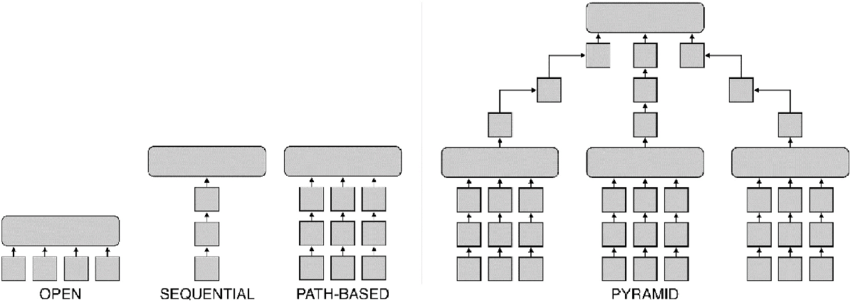
\includegraphics[width=\linewidth]{figures/Puzzle-structures-in-escape-rooms.png}
  \caption{Figure 1: Puzzle structures in escape rooms: a) basic structures: open, sequential and path-based; b) a complex, hybrid structure, such as a pyramid. Squares are puzzles and rectangles are meta-puzzles (adapted from Nicholson, 2015) as cited in \cite{veldkamp_escape_2020}.}
  \Description{Three different puzzle structures and their diagram. Sequential, complex, and pyramid from left to right.}
\end{figure}


\subsection{Cyber Security Awareness Education}

There exist cybersecurity awareness training programmes such as security education, training and awareness (SETA) programmes, but in these SETA programmes cybersecurity knowledge usually increases by 12-17\% and then disappears within a month \cite{pittsburg_state_university_how_2023}. 
These SETA programmes, which are predominant in the professional field, are often seen as tedious and uninspiring by the people who take them \cite{keller_digital_2025}.
Cybersecurity awareness is extremely important, as human factors, such as social engineering tactics, remain the primary point of entry for threat actors, with 60\% coming from phishing \cite{noauthor_threat_2025}. This is also supported by Verizon's 2025 Data Breach Investigation Report (DBIR) which found that 60\% of breaches consist of human involvement \cite{verizon_dbir_2025}. In addition, 66\% of Chief Information Security Officers (CISO) agree that the human factor is their organisation's biggest cyber vulnerability, making it clear that organisations are aware of risks \cite{proofpoint_voice_of_the_ciso_2025}.
The intersection of DEERs and cybersecurity awareness education for non-expert users is under-explored. Most existing EERs target general STEM subjects or medical education, but not necessarily cybersecurity-specific implementations \cite{keller_digital_2025, makri_digital_2021}.
There have been some DEERs for cybersecurity like EyesOnCS by Spatafora et al., although they had some deficiencies, for example immersion challenges, the difficulty being too high, and even their hint system \cite{spatafora_educational_2024}. So, there are some DEERs, but they usually lack evidence of long-term knowledge and act as short-term interventions \cite{gwenhure_gamification_2024}. Additionally, there is not much evidence for actual behavioural change, which is the goal here.




\section{Cyberattack Landscape Analysis}

The selection of threat scenarios in CyberEscape involved a review of the ENISA Threat Landscape 2025 and the 2025 Verizon Data Breach Investigation Report. These reports were analysed to identify attack vectors that impact non-expert users and organisations where the "human factor" is the primary entry element \cite{verizon_dbir_2025, noauthor_threat_2025}. The selected scenarios, phishing, password-based attacks, and unsecured network connections, were prioritised because they do not require special and technical knowledge for a user to fall victim to, yet they can be avoided by behavioural training and scenario-based decision-making \cite{keller_digital_2025, sans_security_awareness_2025}.


\subsection{Phishing and Social Engineering }

Phishing is defined as a fraudulent attempt to trick people into revealing sensitive information, such as login credentials or financial data, by masquerading as a trustworthy entity in electronic communications, usually email or SMS texts \cite{enisa_phishing_2020}. It is the dominant intrusion vector in the current landscape, accounting for 60\% of all observed cases and 74\% of phishing sites even using HTTPS to seem like a secure website \cite{noauthor_threat_2025, enisa_phishing_2020}. 
Phishing targets non-experts by exploiting human nature, using psychological triggers such as urgency, fear, or even authority to provoke an impulsive and emotional response that bypasses rational evaluation \cite{enisa_phishing_2020, keller_digital_2025}. These psychological manipulation tactics used on people to make them act and divulge sensitive information are known as social engineering.
A prevalent type of phishing is "spear phishing" which relies on research on the victims to make the scam appear more authentic leading to one of the mist successful types of attacks \cite{enisa_phishing_2020}.
To avoid these traps, users must be taught to identify specific red flags: suspicious sender addresses, inconsistencies in URLs/hyperlinks, and requests for sensitive information that deviate from professional standards \cite{enisa_phishing_2020}. In this project, this translates into a puzzle mechanic where the player is presented with a simulated email inbox with phishing emails that the player must identify with help of the red flags.


\subsection{Password-based attacks}

Credential attacks involve attempts to obtain unauthorised access to systems by exploiting user passwords through methods such as brute force, the act of systematically guessing credentials, password guessing, and credential stuffing; the act of using leaked passwords from one service to access another \cite{spatafora_educational_2024, verizon_dbir_2025}. These actions are spreading, with credential abuse accounting for 32\% of human element breaches \cite{verizon_dbir_2025}. 
Non-experts remain vulnerable because we humans are historically bad at choosing unfamiliar and complex passwords and frequently reuse them across multiple platforms \cite{spatafora_educational_2024, verizon_dbir_2025}. The teachable elements of this scenario focus on strong passwords such as using long passphrases and mnemonics, the necessity of having unique passwords across platforms, and the role of password managers \cite{sans_security_awareness_2025}. This becomes a puzzle mechanic where players must evaluate a list of credentials to identify weak or reused ones, or must generate a secure password to complete the puzzle.


\subsection{Network Sniffing and Unsecured Connections}

Network sniffing is a technique in which an attack on the same network passively captures data traffic. This occurs most frequently on public Wi-Fi and/or unsecured networks where unencrypted credentials, session keys, and personal information are exposed. According to ENISA, the network server is the attack vector for 64\% of documented vulnerabilities \cite{noauthor_threat_2025}.
Teachable elements for non-experts include recognising the difference between HTTPS and HTTP, the protective roles of Virtual Private Networks (VPNs), the risks of "shadow" connections. In an ER context, this is presented as a scenario where the player must analyse a virtual workplace environment and identify which networks connections are safe by verifying the "lock" icon in a browser, among other possibilities, and which expose data to potential interception.


\section{Escape Room Design}


\subsection{Pedagogical Framework}

The design of CyberEscape is grounded in three core pedagogical pillars: \textbf{constructivism}, \textbf{situated learning}, and \textbf{immediate feedback}.

Firstly, the game uses a constructivism approach, which assumes that learners are not passive recipients of the information being taught, but active participants who construct new knowledge through real-time experiences and interaction with their environment \cite{makri_digital_2021, plass_handbook_2020, plass_foundations_2015}. In CyberEscape, this is achieved by requiring players to solve puzzles requiring understanding of the information given, as well as using it in a real scenario.


Secondly, the design leverages situated learning theory, which argues that knowledge is best acquired in the authentic context where it will later be applied \cite{plass_handbook_2020, plass_foundations_2015, veldkamp_escape_2020}. By embedding cybersecurity challenges within a realistic workplace scenario, such as an email inbox, or a public Wi-Fi setting, the game provides a safe environment for learners to rehearse skills and practice decision-making without the real-world consequences like giving away their data, passwords, or other sensitive information \cite{spatafora_educational_2024, moffett_building_2023}. This scenario-based learning facilitates better knowledge retention and the immediate transfer of skills to the professional environment, which is why immersion is very important, making the learner both realise where these skills and information can be used, keeping them engaged, motivated and if they solve the puzzles even give them a sense of achievement, in conclusion giving them an active learning environment maximising motivation and engagement \cite{makri_digital_2021}.


Lastly, immediate and unambiguous feedback is a critical design element \cite{veldkamp_escape_2020}. The game uses a loop of challenge, response, and feedback, where incorrect decisions are immediately explained to the player, thus correcting him/her when making the mistake instead of waiting until the end when he/she might have already forgotten the mistake. This turns failure into a "learning moment", allowing the player to understand exactly what they missed or did wrong, and reinforcing correct identification strategies before they move on to the next puzzle or challenge.


Together, these three principles ensure that every design choice prioritises active engagement over passive consumption. The game will be single-player, making it lose the communication skills reinforcement, but therefore I focused more strongly on other principles. 




\subsection{Learning Objectives}

The following table outlines the specific learning objectives targeted by the threat scenarios in CyberEscape.

\begin{table}[h!]
\centering
\begin{tabular}{|p{2cm}|p{2cm}|p{4cm}|}
\hline
\textbf{Scenario Name} & \textbf{Puzzle Name} & \textbf{Learning Objective} \\
\hline
Phishing & The Deceptive Inbox & Player can identify at least 3 red flags in a malicious email. \\
\hline
Password Security & The Profile Problem & Player understands what distinguishes a weak from a strong password and why. \\
\hline
Network Sniffing & The Café Connection & Player can identify unsafe connection behaviour on a public network. \\
\hline
\end{tabular}
\caption{Learning Objectives for CyberEscape Scenarios}
\end{table}

 %% Present a clear table — three rows, one per threat scenario, with columns 
 %% for the scenario name, the puzzle name, and the specific learning 
 %% objective. A LaTeX table here is clean and readable.
%% Example structure:
%% ScenarioPuzzleLearning ObjectivePhishingThe Suspicious InboxPlayer can 
%% identify at least 3 red flags in a malicious emailPassword SecurityThe 
%% Locked TerminalPlayer understands what distinguishes a weak from a strong 
%% passwordNetwork SniffingThe Coffee ShopPlayer can identify unsafe 
%% connection behaviour on a public network

\subsection{Narrative and Room Structure}

CyberEscape places the player in everyday situations that anyone who uses the internet will recognise. As this is a proof-of-concept prototype, narrative immersion is kept deliberately light. The priority is the learning outcome that players take from this DEER, as well as the puzzle mechanics. The player will navigate three sequential security checkpoints, each set in a different context from daily (digital) life. There is no previous technical background assumed or required to complete these puzzles. They are aimed at every age group that has a brief understanding of the internet and applications such as email inboxes.


The game follows a sequential structure \cite{veldkamp_escape_2020}: each checkpoint must be completed before the next one becomes accessible, ensuring that the three threat scenarios are encountered in a deliberate order of increasing contextual variety. Each checkpoint opens with a short screen to set the scene, thus establishing the situation without telling the player what red flags to look for until after the completion of the puzzle when the red flags will finally be revealed. The discovery is therefore the learning. Upon completing the puzzle, the player receives an explanatory debrief that consolidates the lesson regardless of the outcome. This means that a player who completes every puzzle in 10 minutes and a player who completes it in 60 minutes or even not at all will both get an explanation as to what the red flags were and are, and what they should look out for, ensuring that every player learns something. 


Figure~\ref{fig:flow} illustrates the overall progression structure 
of CyberEscape.

\begin{figure}[h]
  \centering
  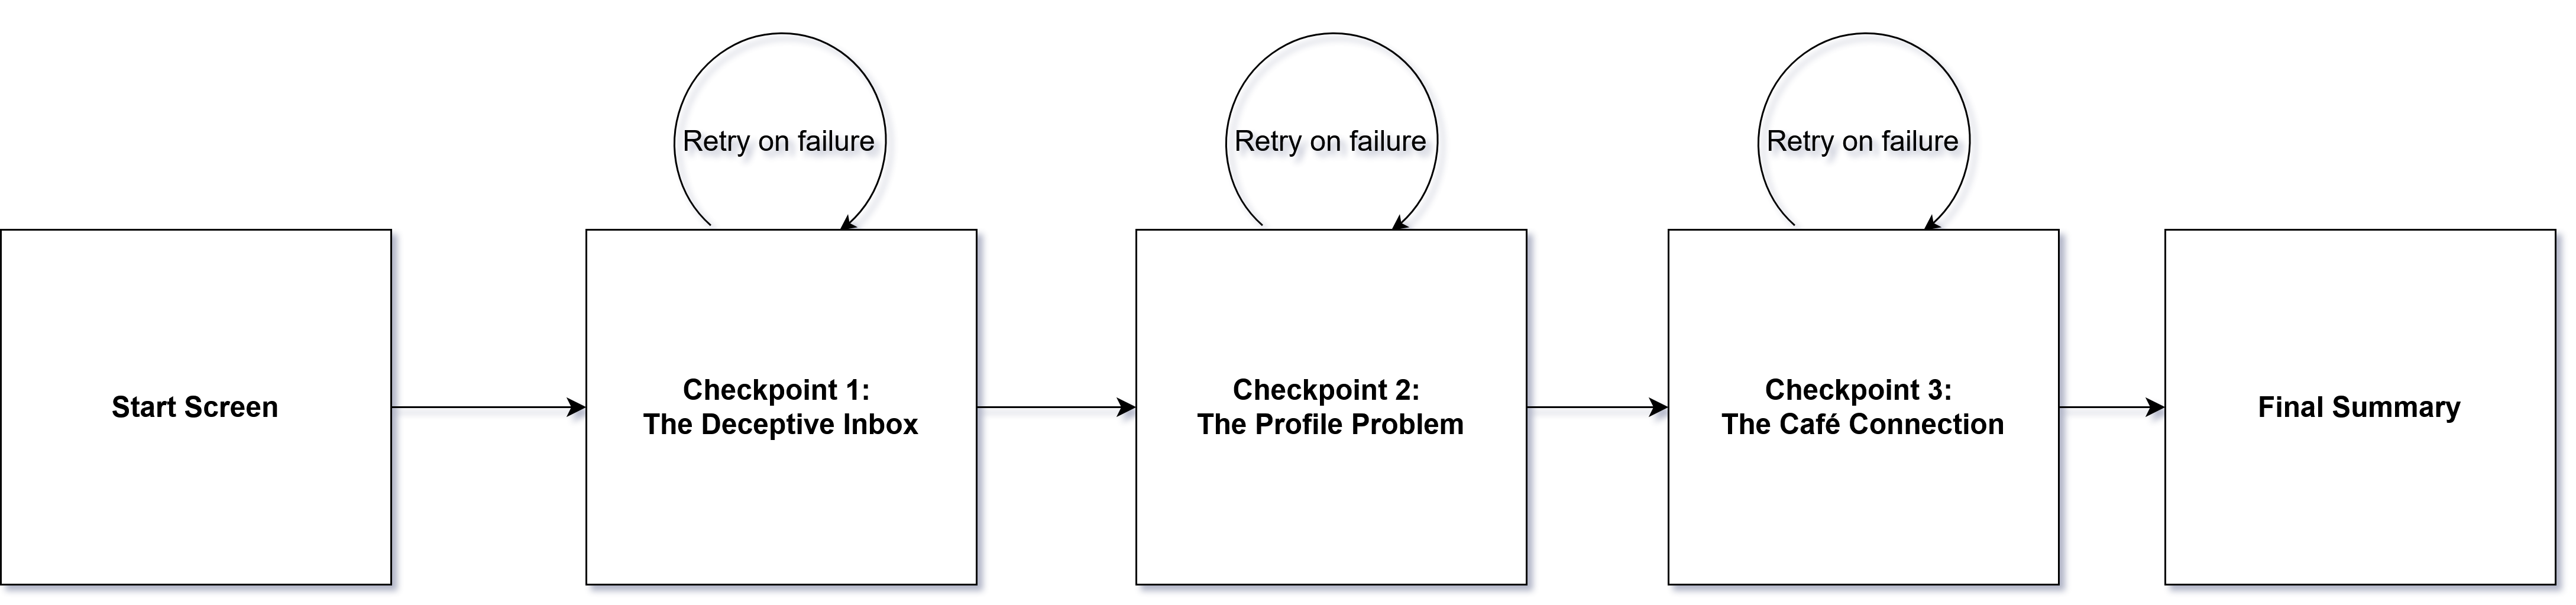
\includegraphics[width=\linewidth]{figures/flow-chart(2).png}
  \caption{CyberEscape sequential progression flow. Each checkpoint 
  must be cleared before the next is accessible. A debrief screen 
  follows every attempt, regardless of outcome.}
  \Description{Flow diagram with five boxes connected by arrows from 
  left to right: Start Screen, Checkpoint 1 The Deceptive Inbox, 
  Checkpoint 2 The Profile Problem, Checkpoint 3 The Café Connection, 
  Final Summary Screen. Each checkpoint box has a small looping arrow 
  indicating retry on failure.}
  \label{fig:flow}
\end{figure}


Table~\ref{tab:structure} summarises the three checkpoints, their corresponding threat scenario, and their real-world setting.


\begin{table}[h!]
\centering
\begin{tabular}{|p{0.6cm}|p{2cm}|p{2.2cm}|p{2cm}|}
\hline
\textbf{No.} & \textbf{Checkpoint} & \textbf{Threat Scenario} & 
\textbf{Setting} \\
\hline
1 & The Deceptive Inbox & Phishing \& Social Engineering & 
Personal or work email client \\
\hline
2 & The Profile Problem & Password-Based Attacks & 
Social media profile and login screen \\
\hline
3 & The Café Connection & Network Sniffing & 
Café during a break \\
\hline
\end{tabular}
\caption{CyberEscape checkpoint structure and sequential 
progression order.}
\label{tab:structure}
\end{table}


\subsection{Puzzle Designs}

\subsubsection{Checkpoint 1: The Deceptive Inbox}

The player is presented with a simulated email client with the screen divided into two panels. The left panel shows five email previews, each displaying the sender address and subject line. Clicking a preview opens the full email in the right panel, showing the From, To, Subject, and message body fields. The email pool is drawn from a larger data set containing four legitimate emails and two phishing emails; each session selects three legitimate emails at random and always includes both phishing emails, giving five in total.

The player must classify each email as \textbf{PHISHING} or \textbf{SAFE} using two buttons at the bottom of the viewer. Once all five are labelled, pressing the Enter key submits the answers. Both phishing emails contain identifiable red flags grounded in real attack patterns \cite{enisa_phishing_2020}. The first comes from \textbf{support@rnicrosoft.com}, where the character combination ``rn'' visually mimics the letter ``m'', a technique known as typosquatting. Its subject threatens account suspension within 24 hours and asks the player to click a verification link. The second arrives from \textbf{security@ing-lU.com}, falsely claiming a suspicious transaction and demanding verification via a link that does not match any official domain.

Any misclassification triggers a three-second retry screen and resets the puzzle with a newly shuffled email set. Players who classify all five correctly advance to the next checkpoint which explains what this new puzzle is about and what to do. 


\subsubsection{Checkpoint 2: The Profile Problem}

The screen is divided into two panels. The left panel displays a fictional social media profile belonging to Sarah Mitchell (\textbf{@sarah\_m\_lux}), showing her birthday, location, dog's name, favourite football club, and favourite player, along recent "posts" that repeat the same details. The right panel hosts the interactive puzzle, which runs in two sequential phases.

In Part A, the player is shown six password candidates, three derived from Sarah's profile and three not, and must identify which one she is most likely to be using. In Part B, the player is shown four candidates and must identify the genuinely strong one. Each phase requires the player to confirm their selection before receiving feedback.

In Part A, any password that draws directly from the visible profile information is accepted as correct; examples include
\textbf{Biscuit2022}, \textbf{Chelsea1990}, or \textbf{Sarah\_14March}. The point is not a single right answer, but
that the player demonstrates understanding of why personal information makes passwords predictable \cite{spatafora_educational_2024, verizon_dbir_2025}. In Part B, the only correct answer is \textbf{Lamp!River93Desk}, a passphrase of three unrelated words combined with a number and a symbol. Selecting a non-personal password in Part A or a weak one in Part B resets that phase and shows a brief explanation before the player tries again. Once again, upon successful completion, the next state is loaded, which is the introduction screen for puzzle 3, which explains what it is about and how to solve it. 


\subsubsection{Checkpoint 3: The Café Connection}

The player is told that they are on a break in a café and need to quickly cheque something online. The checkpoint runs in three sequential steps, each with its own instruction and a set of selectable options.

Step 1 presents four Wi-Fi networks. Three are unsafe: an open network with no password, a network labelled ``Guest'' that is also unencrypted, and an unidentified personal hotspot. The correct choice is the single WPA2 password-protected network. Selecting an unsafe option shows an explanation specific to that network and resets the selection; the player cannot advance until the correct network is chosen. 
Step 2 displays two simulated browser address bars. One shows \textbf{http://mybank.lu/login} with a warning indicator; the other shows \textbf{https://mybank.lu/login} with a padlock "icon". Again, an incorrect selection shows an explanation and resets before the player can advance. 
Step 3 presents six daily online actions and asks the player to mark each as \textbf{SAFE} or \textbf{RISKY}. Reading the news or checking the weather are safe; logging into online banking, entering credit card details, or sending work emails containing private content are risky even on a nominally protected network.

The three key takeaways: how open networks expose unencrypted traffic, what the HTTPS padlock guarantees, and which actions should be avoided on any public connection \cite{noauthor_threat_2025}.


\section{Prototype Implementation}

\subsection{Technology Stack}

CyberEscape is implemented entirely in Python, chosen for its readability and the availability of the Pygame library. The prototype runs on Python 3.13 and depends on a single third-party library, Pygame 2.6.1, which provides hardware-accelerated 2D rendering, event handling, font rendering, and a fixed-rate game loop. No other external dependencies are required. I have also chosen PyGame because of my experience with it in high school, where Python and PyGame were my main programme for my Computer Science lectures. 

The game launches in full-screen mode and reads the display resolution at startup, computing all layout dimensions dynamically so that the interface scales to any screen. All puzzle content, including email text, password candidates, network configurations, and action labels, is stored as plain Python data structures in a dedicated constants module. This separation of content from rendering logic means that the puzzle data can be modified or extended without touching the drawing code.

\subsection{System Architecture}

The application is built around a flat state machine coordinated by a central game loop in \texttt{main.py}. At any given moment, the application is in exactly one of eleven named states: 

\texttt{intro}, \texttt{puzzle1\_intro}, \texttt{puzzle1}, \texttt{puzzle2\_intro}, \texttt{puzzle2}, 

\texttt{puzzle3\_intro}, \texttt{puzzle3}, \texttt{summary1}, \texttt{summary2}, \texttt{summary3}, and \texttt{retry}. State transitions are triggered by the return value of the active module's \texttt{handle()} function.

Each module, \texttt{Menu.py}, \texttt{puzzle1.py}, \texttt{puzzle2.py}, \texttt{puzzle3.py}, and \texttt{checkpoints.py}, exposes three module-level functions with a uniform interface: \texttt{setup()} initialises or resets the module's state; \texttt{handle(event)} processes a single Pygame event and returns either \texttt{None} (no transition) or a string identifying the next state; and \texttt{draw(screen)} renders the current frame. This keeps the main loop free of module-specific logic.

A shared utility module, \texttt{txt\_rect.py}, provides two dynamic text-rendering functions that wrap a string to fit inside a given rectangle and scale the font size downward until the full text fits, removing the need to manually calibrate the font sizes. A 15-minute countdown timer is maintained in the main loop; when it expires, the game advances directly to the summary screens regardless of the player's current progress, ensuring every player receives the full educational debrief.

\subsection{Implemented Mechanics}

Puzzle 1 implements a two-panel email client simulation. Each email is represented as an object that contains the sender, recipient, subject, body text, and a \texttt{flagged} attribute (True, False, or None if unclassified). The player assigns each email a classification using the PHISHING or SAFE buttons; submission is blocked until all five carry a label. Pressing Enter evaluates each classification against its ground-truth value and either advances the game or triggers a retry with a reshuffled email set.

Puzzle 2 implements a two-phase password evaluation mechanic in conjunction with a persistent social media profile panel. In Phase A, six password candidates are displayed as selectable buttons, and the player must identify one derivable from the visible profile information. In Phase B, four candidates are shown and the player must select the strongest one. Each phase requires an explicit confirmation click before feedback is shown; incorrect selections reset only the current phase, allowing the player to retry after reading the explanation.

Puzzle 3 is structured as three sequential micro-tasks within a single checkpoint. Phase 1 uses a card-based network selector with one option per network; Phase 2 simulates two browser address bars with colour-coded security indicators; Phase 3 uses a row-based interface where each of the six action rows has dedicated SAFE and RISKY buttons. A module-level variable (\texttt{retry\_phase}) records which phase failed, so that a Phase 3 retry restarts only from Phase 3 rather than from the beginning of the checkpoint.

All three puzzles share the same interaction pattern: select an option, confirm, receive immediate feedback, and either advance or correct the answer. Post-checkpoint debrief screens rendered by the \texttt{checkpoints} module consolidate the educational content for each threat scenario, and are shown to every player regardless of performance.

\section{Conclusion}

This paper has presented CyberEscape, a digital educational escape room prototype designed to teach foundational cybersecurity awareness to non-expert users through active, scenario-based decision-making. Grounded in constructivist and situated learning theory, the prototype delivers three puzzle-based checkpoints that cover phishing identification, password security, and safe behaviour on public Wi-Fi networks. The DEER concludes with an explanatory debrief screen, ensuring that every player receives the educational content regardless of their in-game performance, even if the game was not completed in the due time.

The implementation demonstrates that Python and Pygame provide a sufficient foundation for a functional and modular DEER prototype, with dynamic content randomisation, resolution-independent layout, and a clean separation between game content and rendering logic.

Several limitations remain. The prototype has not been evaluated with real users, so claims about learning effectiveness are hypothetical at this stage. The single-player format, while appropriate for a proof-of-concept, removes the social interaction and collaborative problem-solving that characterise physical escape rooms and that some research associates with greater engagement and retention \cite{veldkamp_escape_2020, jarvelainen_relativity_2023}. Narrative immersion is intentionally minimal and could be substantially deepened in a more complete implementation. The current puzzle set also covers only three of the many cybersecurity threat scenarios relevant to non-expert users.

Future work should prioritise a formal user evaluation with a representative sample to assess both perceived engagement and actual learning outcomes. Extending the puzzle set to additional scenarios, such as social media oversharing or two-factor authentication, would broaden the educational scope. A multiplayer mode would allow for investigation of whether collaborative play produces stronger outcomes than the current single-player format, in line with findings from the broader educational literature on escape rooms \cite{makri_digital_2021, veldkamp_escape_2020}.

\appendix

\section{Disclosure of Generative AI Use}

In accordance with the University of Luxembourg Guidelines on the Use  of Generative AI Tools for Learning and Teaching (2025), I want to disclose the following use of AI tools in the preparation of this report.

\subsection*{Claude (Anthropic)}

Claude was used for two distinct purposes. First, it provided coding assistance during the implementation of the prototype. Rather than generating the application as a whole, Claude was primarily consulted for guidance on how to implement specific features or how to structure certain components (for example, the implementation of individual puzzles or aspects of the programme architecture). The prototype itself was written by me, including the design choices and the overall behaviour of the application. Claude's suggestions were selectively incorporated where appropriate, while all code was reviewed, tested, and adapted manually by me.

Second, Claude was consulted during the structural planning of this report, specifically for guidance on how to organise the sections and subsections in accordance with academic writing conventions. The intellectual content of each section, including the literature review, the threat scenarios selected, the design decisions made, and the arguments presented, is my own work. Claude did not generate any factual claims, citations, or analysis included in this report.

\subsection*{NotebookLM (Google)}

NotebookLM was used as a source management and summarisation tool during the literature review phase. Uploaded research papers were queried to assist in organising and cross-referencing sources, and the tool was occasionally used to help rephrase passages for clarity while preserving factual accuracy. All rephrased content was reviewed and verified against the original sources by me, before including it in the report.

\subsection*{Impact on the Work}

The use of these tools affected the presentation and organisation of this work, but not its substance. The research questions, the selection of threat scenarios, the pedagogical design choices, and the conclusions drawn are the result of my own reading, thinking, and decision-making, as well as the help of my supervisor Professor Muriel-Larissa FRANK. AI assistance was used to improve clarity, accelerate structuring, and support technical implementation, not to replace the intellectual work required by the project.

\bibliographystyle{ACM-Reference-Format}
\bibliography{references}

\end{document}
\endinput
%%
%% End of file `sample-sigconf.tex'.

%% \section{Authors and Affiliations}

%% Each author must be defined separately for accurate metadata
%% identification.  As an exception, multiple authors may share one
%% affiliation. Authors' names should not be abbreviated; use full first
%% names wherever possible. Include authors' e-mail addresses whenever
%% possible.

%% Grouping authors' names or e-mail addresses, or providing an ``e-mail
%% alias,'' as shown below, is not acceptable:
%% \begin{verbatim}
%%  \author{Brooke Aster, David Mehldau}
%%  \email{dave,judy,steve@university.edu}
%%  \email{firstname.lastname@phillips.org}
%% \end{verbatim}

%% The \verb|authornote| and \verb|authornotemark| commands allow a note
%% to apply to multiple authors --- for example, if the first two authors
%% of an article contributed equally to the work.

%% If your author list is lengthy, you must define a shortened version of
% the list of authors to be used in the page headers, to prevent
% overlapping text. The following command should be placed just after
% the last \verb|\author{}| definition:
% \begin{verbatim}
%   \renewcommand{\shortauthors}{McCartney, et al.}
% \end{verbatim}
% Omitting this command will force the use of a concatenated list of all
% of the authors' names, which may result in overlapping text in the
% page headers.

% The article template's documentation, available at
% \url{https://www.acm.org/publications/proceedings-template}, has a
% complete explanation of these commands and tips for their effective
% use.

% Note that authors' addresses are mandatory for journal articles.

% \section{Rights Information}

% Authors of any work published by ACM will need to complete a rights
% form. Depending on the kind of work, and the rights management choice
% made by the author, this may be copyright transfer, permission,
% license, or an OA (open access) agreement.

% Regardless of the rights management choice, the author will receive a
% copy of the completed rights form once it has been submitted. This
% form contains \LaTeX\ commands that must be copied into the source
% document. When the document source is compiled, these commands and
% their parameters add formatted text to several areas of the final
% document:
% \begin{itemize}
% \item the ``ACM Reference Format'' text on the first page.
% \item the ``rights management'' text on the first page.
% \item the conference information in the page header(s).
% \end{itemize}

% Rights information is unique to the work; if you are preparing several
% works for an event, make sure to use the correct set of commands with
% each of the works.

% The ACM Reference Format text is required for all articles over one
% page in length, and is optional for one-page articles (abstracts).

% \section{CCS Concepts and User-Defined Keywords}

% Two elements of the ``acmart'' document class provide powerful
% taxonomic tools for you to help readers find your work in an online
% search.

% The ACM Computing Classification System ---
% \url{https://www.acm.org/publications/class-2012} --- is a set of
% classifiers and concepts that describe the computing
% discipline. Authors can select entries from this classification
% system, via \url{https://dl.acm.org/ccs/ccs.cfm}, and generate the
% commands to be included in the \LaTeX\ source.

% User-defined keywords are a comma-separated list of words and phrases
% of the authors' choosing, providing a more flexible way of describing
% the research being presented.

% CCS concepts and user-defined keywords are required for for all
% articles over two pages in length, and are optional for one- and
% two-page articles (or abstracts).

% \section{Sectioning Commands}

% Your work should use standard \LaTeX\ sectioning commands:
% \verb|\section|, \verb|\subsection|, \verb|\subsubsection|,
% \verb|\paragraph|, and \verb|\subparagraph|. The sectioning levels up to
% \verb|\subsubsection| should be numbered; do not remove the numbering
% from the commands.

% Simulating a sectioning command by setting the first word or words of
% a paragraph in boldface or italicized text is {\bfseries not allowed.}

% Below are examples of sectioning commands.

% \subsection{Subsection}
% \label{sec:subsection}

% This is a subsection.

% \subsubsection{Subsubsection}
% \label{sec:subsubsection}

% This is a subsubsection.

% \paragraph{Paragraph}

% This is a paragraph.

% \subparagraph{Subparagraph}

% This is a subparagraph.

% \section{Tables}

% The ``\verb|acmart|'' document class includes the ``\verb|booktabs|''
% package --- \url{https://ctan.org/pkg/booktabs} --- for preparing
% high-quality tables.

% Table captions are placed {\itshape above} the table.

% Because tables cannot be split across pages, the best placement for
% them is typically the top of the page nearest their initial cite.  To
% ensure this proper ``floating'' placement of tables, use the
% environment \textbf{table} to enclose the table's contents and the
% table caption.  The contents of the table itself must go in the
% \textbf{tabular} environment, to be aligned properly in rows and
% columns, with the desired horizontal and vertical rules.  Again,
% detailed instructions on \textbf{tabular} material are found in the
% \textit{\LaTeX\ User's Guide}.

% Immediately following this sentence is the point at which
% Table~\ref{tab:freq} is included in the input file; compare the
% placement of the table here with the table in the printed output of
% this document.

% \begin{table}
%   \caption{Frequency of Special Characters}
%   \label{tab:freq}
%   \begin{tabular}{ccl}
%     \toprule
%     Non-English or Math&Frequency&Comments\\
%     \midrule
%     \O & 1 in 1,000& For Swedish names\\
%     $\pi$ & 1 in 5& Common in math\\
%     \$ & 4 in 5 & Used in business\\
%     $\Psi^2_1$ & 1 in 40,000& Unexplained usage\\
%   \bottomrule
% \end{tabular}
% \end{table}

% To set a wider table, which takes up the whole width of the page's
% live area, use the environment \textbf{table*} to enclose the table's
% contents and the table caption.  As with a single-column table, this
% wide table will ``float'' to a location deemed more
% desirable. Immediately following this sentence is the point at which
% Table~\ref{tab:commands} is included in the input file; again, it is
% instructive to compare the placement of the table here with the table
% in the printed output of this document.

% \begin{table*}
%   \caption{Some Typical Commands}
%   \label{tab:commands}
%   \begin{tabular}{ccl}
%     \toprule
%     Command &A Number & Comments\\
%     \midrule
%     \texttt{{\char'134}author} & 100& Author \\
%     \texttt{{\char'134}table}& 300 & For tables\\
%     \texttt{{\char'134}table*}& 400& For wider tables\\
%     \bottomrule
%   \end{tabular}
% \end{table*}

% Always use midrule to separate table header rows from data rows, and
% use it only for this purpose. This enables assistive technologies to
% recognise table headers and support their users in navigating tables
% more easily.

% \section{Math Equations}
% You may want to display math equations in three distinct styles:
% inline, numbered or non-numbered display.  Each of the three are
% discussed in the next sections.

% \subsection{Inline (In-text) Equations}
% A formula that appears in the running text is called an inline or
% in-text formula.  It is produced by the \textbf{math} environment,
% which can be invoked with the usual
% \texttt{{\char'134}begin\,\ldots{\char'134}end} construction or with
% the short form \texttt{\$\,\ldots\$}. You can use any of the symbols
% and structures, from $\alpha$ to $\omega$, available in
% \LaTeX~\cite{Lamport:LaTeX}; this section will simply show a few
% examples of in-text equations in context. Notice how this equation:
% \begin{math}
%   \lim_{n\rightarrow \infty}x=0
% \end{math},
% set here in in-line math style, looks slightly different when
% set in display style.  (See next section).

% \subsection{Display Equations}
% A numbered display equation---one set off by vertical space from the
% text and centered horizontally---is produced by the \textbf{equation}
% environment. An unnumbered display equation is produced by the
% \textbf{displaymath} environment.

% Again, in either environment, you can use any of the symbols and
% structures available in \LaTeX\@; this section will just give a couple
% of examples of display equations in context.  First, consider the
% equation, shown as an inline equation above:
% \begin{equation}
%   \lim_{n\rightarrow \infty}x=0
% \end{equation}
% Notice how it is formatted somewhat differently in
% the \textbf{displaymath}
% environment.  Now, we'll enter an unnumbered equation:
% \begin{displaymath}
%   \sum_{i=0}^{\infty} x + 1
% \end{displaymath}
% and follow it with another numbered equation:
% \begin{equation}
%   \sum_{i=0}^{\infty}x_i=\int_{0}^{\pi+2} f
% \end{equation}
% just to demonstrate \LaTeX's able handling of numbering.

% \section{Figures}

% The ``\verb|figure|'' environment should be used for figures. One or
% more images can be placed within a figure. If your figure contains
% third-party material, you must clearly identify it as such, as shown
% in the example below.
% \begin{figure}[h]
%   \centering
%   \includegraphics[width=\linewidth]{sample-franklin}
%   \caption{1907 Franklin Model D roadster. Photograph by Harris \&
%     Ewing, Inc. [Public domain], via Wikimedia
%     Commons. (\url{https://goo.gl/VLCRBB}).}
%   \Description{A woman and a girl in white dresses sit in an open car.}
% \end{figure}

% Your figures should contain a caption which describes the figure to
% the reader.

% Figure captions are placed {\itshape below} the figure.

% Every figure should also have a figure description unless it is purely
% decorative. These descriptions convey what’s in the image to someone
% who cannot see it. They are also used by search engine crawlers for
% indexing images, and when images cannot be loaded.

% A figure description must be unformatted plain text less than 2000
% characters long (including spaces).  {\bfseries Figure descriptions
%   should not repeat the figure caption – their purpose is to capture
%   important information that is not already provided in the caption or
%   the main text of the paper.} For figures that convey important and
% complex new information, a short text description may not be
% adequate. More complex alternative descriptions can be placed in an
% appendix and referenced in a short figure description. For example,
% provide a data table capturing the information in a bar chart, or a
% structured list representing a graph.  For additional information
% regarding how best to write figure descriptions and why doing this is
% so important, please see
% \url{https://www.acm.org/publications/taps/describing-figures/}.

% \subsection{The ``Teaser Figure''}

% A ``teaser figure'' is an image, or set of images in one figure, that
% are placed after all author and affiliation information, and before
% the body of the article, spanning the page. If you wish to have such a
% figure in your article, place the command immediately before the
% \verb|\maketitle| command:
% \begin{verbatim}
%   \begin{teaserfigure}
%     \includegraphics[width=\textwidth]{sampleteaser}
%     \caption{figure caption}
%     \Description{figure description}
%   \end{teaserfigure}
% \end{verbatim}

% \section{Citations and Bibliographies}

% The use of \BibTeX\ for the preparation and formatting of one's
% references is strongly recommended. Authors' names should be complete
% --- use full first names (``Donald E. Knuth'') not initials
% (``D. E. Knuth'') --- and the salient identifying features of a
% reference should be included: title, year, volume, number, pages,
% article DOI, etc.

% The bibliography is included in your source document with these two
% commands, placed just before the \verb|\end{document}| command:
% \begin{verbatim}
%   \bibliographystyle{ACM-Reference-Format}
%   \bibliography{bibfile}
% \end{verbatim}
% where ``\verb|bibfile|'' is the name, without the ``\verb|.bib|''
% suffix, of the \BibTeX\ file.

% Citations and references are numbered by default. A small number of
% ACM publications have citations and references formatted in the
% ``author year'' style; for these exceptions, please include this
% command in the {\bfseries preamble} (before the command
% ``\verb|\begin{document}|'') of your \LaTeX\ source:
% \begin{verbatim}
%   \citestyle{acmauthoryear}
% \end{verbatim}


%   Some examples.  A paginated journal article \cite{Abril07}, an
%   enumerated journal article \cite{Cohen07}, a reference to an entire
%   issue \cite{JCohen96}, a monograph (whole book) \cite{Kosiur01}, a
%   monograph/whole book in a series (see 2a in spec. document)
%   \cite{Harel79}, a divisible-book such as an anthology or compilation
%   \cite{Editor00} followed by the same example, however we only output
%   the series if the volume number is given \cite{Editor00a} (so
%   Editor00a's series should NOT be present since it has no vol. no.),
%   a chapter in a divisible book \cite{Spector90}, a chapter in a
%   divisible book in a series \cite{Douglass98}, a multi-volume work as
%   book \cite{Knuth97}, a couple of articles in a proceedings (of a
%   conference, symposium, workshop for example) (paginated proceedings
%   article) \cite{Andler79, Hagerup1993}, a proceedings article with
%   all possible elements \cite{Smith10}, an example of an enumerated
%   proceedings article \cite{VanGundy07}, an informally published work
%   \cite{Harel78}, a couple of preprints \cite{Bornmann2019,
%     AnzarootPBM14}, a doctoral dissertation \cite{Clarkson85}, a
%   master's thesis: \cite{anisi03}, an online document / world wide web
%   resource \cite{Thornburg01, Ablamowicz07, Poker06}, a video game
%   (Case 1) \cite{Obama08} and (Case 2) \cite{Novak03} and \cite{Lee05}
%   and (Case 3) a patent \cite{JoeScientist001}, work accepted for
%   publication \cite{rous08}, 'YYYYb'-test for prolific author
%   \cite{SaeediMEJ10} and \cite{SaeediJETC10}. Other cites might
%   contain 'duplicate' DOI and URLs (some SIAM articles)
%   \cite{Kirschmer:2010:AEI:1958016.1958018}. Boris / Barbara Beeton:
%   multi-volume works as books \cite{MR781536} and \cite{MR781537}. A
%   presentation~\cite{Reiser2014}. An article under
%   review~\cite{Baggett2025}. A
%   couple of citations with DOIs:
%   \cite{2004:ITE:1009386.1010128,Kirschmer:2010:AEI:1958016.1958018}. Online
%   citations: \cite{TUGInstmem, Thornburg01, CTANacmart}.
%   Artifacts: \cite{R} and \cite{UMassCitations}.

% \section{Acknowledgments}

% Identification of funding sources and other support, and thanks to
% individuals and groups that assisted in the research and the
% preparation of the work should be included in an acknowledgment
% section, which is placed just before the reference section in your
% document.

% This section has a special environment:
% \begin{verbatim}
%   \begin{acks}
%   ...
%   \end{acks}
% \end{verbatim}
% so that the information contained therein can be more easily collected
% during the article metadata extraction phase, and to ensure
% consistency in the spelling of the section heading.

% Authors should not prepare this section as a numbered or unnumbered {\verb|\section|}; please use the ``{\verb|acks|}'' environment.

% \section{Appendices}

% If your work needs an appendix, add it before the
% ``\verb|\end{document}|'' command at the conclusion of your source
% document.

% Start the appendix with the ``\verb|appendix|'' command:
% \begin{verbatim}
%   \appendix
% \end{verbatim}
% and note that in the appendix, sections are lettered, not
% numbered. This document has two appendices, demonstrating the section
% and subsection identification method.

% \section{Multi-language papers}

% Papers may be written in languages other than English or include
% titles, subtitles, keywords and abstracts in different languages (as a
% rule, a paper in a language other than English should include an
% English title and an English abstract).  Use \verb|language=...| for
% every language used in the paper.  The last language indicated is the
% main language of the paper.  For example, a French paper with
% additional titles and abstracts in English and German may start with
% the following command
% \begin{verbatim}
% \documentclass[sigconf, language=english, language=german,
%                language=french]{acmart}
% \end{verbatim}

% The title, subtitle, keywords and abstract will be typeset in the main
% language of the paper.  The commands \verb|\translatedXXX|, \verb|XXX|
% begin title, subtitle and keywords, can be used to set these elements
% in the other languages.  The environment \verb|translatedabstract| is
% used to set the translation of the abstract.  These commands and
% environment have a mandatory first argument: the language of the
% second argument.  See \verb|sample-sigconf-i13n.tex| file for examples
% of their usage.

% \section{SIGCHI Extended Abstracts}

% The ``\verb|sigchi-a|'' template style (available only in \LaTeX\ and
% not in Word) produces a landscape-orientation formatted article, with
% a wide left margin. Three environments are available for use with the
% ``\verb|sigchi-a|'' template style, and produce formatted output in
% the margin:
% \begin{description}
% \item[\texttt{sidebar}:]  Place formatted text in the margin.
% \item[\texttt{marginfigure}:] Place a figure in the margin.
% \item[\texttt{margintable}:] Place a table in the margin.
% \end{description}

% %%
% %% The acknowledgments section is defined using the "acks" environment
% %% (and NOT an unnumbered section). This ensures the proper
% %% identification of the section in the article metadata, and the
% %% consistent spelling of the heading.
% \begin{acks}
% To Robert, for the bagels and explaining CMYK and color spaces.
% \end{acks}

% %%
% %% The next two lines define the bibliography style to be used, and
% %% the bibliography file.
% \bibliographystyle{ACM-Reference-Format}
% \bibliography{sample-base}


% %%
% %% If your work has an appendix, this is the place to put it.
% \appendix

% \section{Research Methods}

% \subsection{Part One}

% Lorem ipsum dolor sit amet, consectetur adipiscing elit. Morbi
% malesuada, quam in pulvinar varius, metus nunc fermentum urna, id
% sollicitudin purus odio sit amet enim. Aliquam ullamcorper eu ipsum
% vel mollis. Curabitur quis dictum nisl. Phasellus vel semper risus, et
% lacinia dolor. Integer ultricies commodo sem nec semper.

% \subsection{Part Two}

% Etiam commodo feugiat nisl pulvinar pellentesque. Etiam auctor sodales
% ligula, non varius nibh pulvinar semper. Suspendisse nec lectus non
% ipsum convallis congue hendrerit vitae sapien. Donec at laoreet
% eros. Vivamus non purus placerat, scelerisque diam eu, cursus
% ante. Etiam aliquam tortor auctor efficitur mattis.

% \section{Online Resources}

% Nam id fermentum dui. Suspendisse sagittis tortor a nulla mollis, in
% pulvinar ex pretium. Sed interdum orci quis metus euismod, et sagittis
% enim maximus. Vestibulum gravida massa ut felis suscipit
% congue. Quisque mattis elit a risus ultrices commodo venenatis eget
% dui. Etiam sagittis eleifend elementum.

% Nam interdum magna at lectus dignissim, ac dignissim lorem
% rhoncus. Maecenas eu arcu ac neque placerat aliquam. Nunc pulvinar
% massa et mattis lacinia.